\phantomsection
\addcontentsline{toc}{section}{Introduction}
\section*{Introduction}
Afin de mener à bien la conception et le développement d'une application mobile de gestion des événements interactifs, il est essentiel de réaliser une collecte d'informations sur les travaux existants et les solutions déjà mises en place dans ce domaine. Ce chapitre sera consacré, dans un premier temps, à une clarification conceptuelle des notions clés liées aux événements interactifs et à leur gestion. Ensuite, une étude des applications existantes sera menée afin d'identifier leurs fonctionnalités, leurs forces et leurs limites. Cette analyse permettra de mieux cerner les défis actuels et de poser les bases pour le développement d'une solution optimisée et adaptée aux besoins des utilisateurs.
 \section{Clarification conceptuelle}
\subsection{ Application mobile}
\subsubsection{Definition}
Les applications mobiles, sont des logiciels développés spécifiquement pour les systèmes d'exploitation mobiles. Elles sont, ensuite, accessibles au téléchargement depuis les plateformes de distribution (App Store et Google Play Store). On utilise des langages de programmation et des outils adaptés à chaque plateforme ou des approches multiplateformes permettant de cibler plusieurs systèmes avec une base de code unique.

L'application s'exécute sur le dispositif mobile et peut utiliser ses ressources, telles que le GPS, la caméra, et les capteurs de mouvement, afin d'offrir des fonctionnalités interactives et personnalisées. Elles communiquent souvent avec des serveurs distants via internet pour récupérer des données, mettre à jour leur contenu, ou exécuter des tâches qui nécessitent de la puissance de calcul supplémentaire ou un accès à des bases de données volumineuses \cite{definition-application-mobile}.

\begin{figure}[H]
   \centering
   
\includegraphics[scale=0.3]{images/application.png}
   \caption{Une application mobile}
   \label{fig:application-mobile-definition}
\end{figure}


\subsubsection{ Les différents types d'applications mobiles}
Techniquement parlant, il existe trois types d'applications mobiles que tout utilisateur peut rencontrer :
\begin{figure}[H]
   \centering
   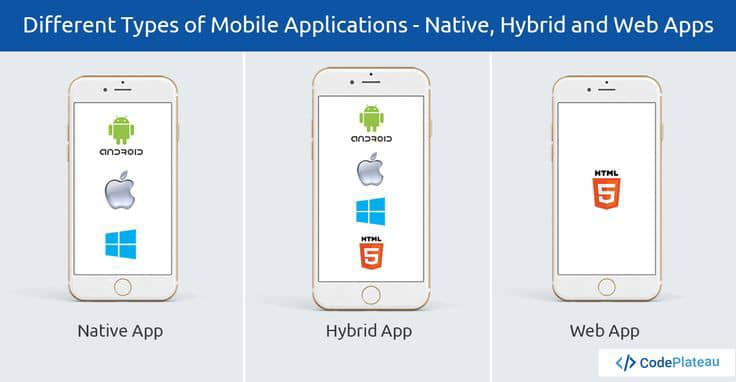
\includegraphics[scale=0.5]{images/78.jpg}
   \caption{ Les différents types d'application mobile}
   \label{fig:types-applications-schema}
\end{figure}
